\documentclass[11pt]{article}
\usepackage{setspace}
\usepackage[a4paper,margin=1in]{geometry}
\geometry{margin=0.85in}
\setstretch{1.0}
\usepackage{graphicx}
\usepackage{array}
\usepackage{setspace}
\usepackage{parskip}
\usepackage{ragged2e}

\pagestyle{empty}
\setstretch{1.05}

\begin{document}


% Title
\begin{center}
    {\Large \textbf{Job Application}} \\[3cm]
    
    {\Huge \textbf{Zhongli Wang}} \\[0.4cm]
    
    {\LARGE Application for Quantitative Researcher}
\end{center}

\vspace{0.6cm}

% Large picture in the middle
\begin{center}
    \IfFileExists{../zhongli-wang-profile.jpg}{
        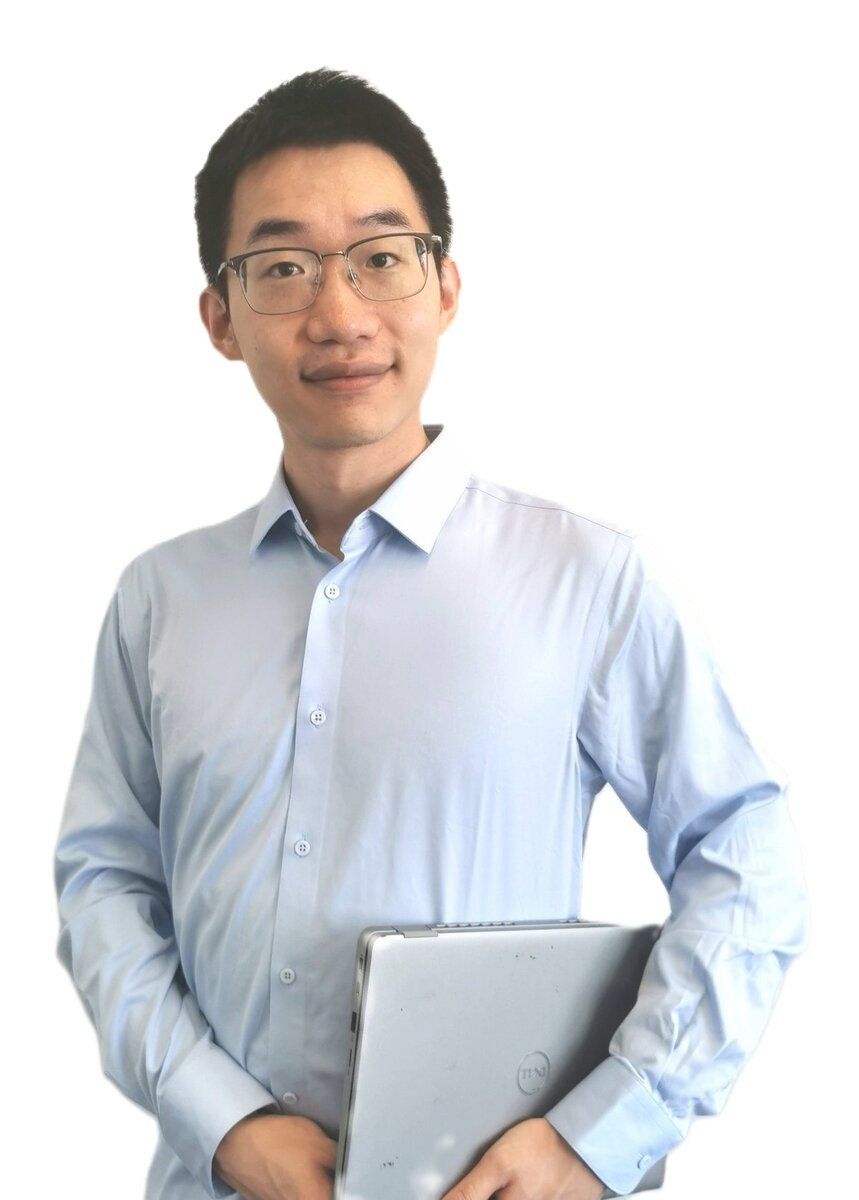
\includegraphics[
            width=0.55\textwidth,
            height=0.45\textheight,
            keepaspectratio
        ]{../zhongli-wang-profile.jpg}
    }{
        \vspace{0.45\textheight}
    }
\end{center}

\vspace{0.7cm}

% \vspace{3cm}


% Personal details
\begin{center}
\renewcommand{\arraystretch}{1.35}
\begin{tabular}{>{\bfseries}p{4.2cm} p{8.5cm}}


Address: & Astastrasse 22, 33617 Bielefeld, Germany \\

Number: & +49 160 9541 6015 \\

Email: & nkwangzhongli@gmail.com \\
\end{tabular}
\end{center}

\vfill

% \begin{center}
%     \small Last updated: \today
% \end{center}
\newpage
\enlargethispage{4\baselineskip}

\begin{flushright}
Zhongli Wang \\
Astastrasse 22 \\
33617 Bielefeld\\
Germany \\
\end{flushright}

\vspace{0.1cm}

\vspace{0.1cm}

\noindent
Mathematica \\
600 Alexander Park \\
Princeton, NJ 08540, USA

\vspace{0.12cm}

\noindent
\textbf{Application for Quantitative Researcher}

\vspace{0.1cm}

\noindent Dear Mathematica recruiting team,

I recently completed my Ph.D. in Economics in a joint program between Bielefeld University and UCSC Milan,
successfully defending my dissertation on September 21, 2026.
I also hold an M.A. in Business and Economics with a major in Banking and Finance and a minor in Data Science.
My doctoral research applies computational and econometric methods to questions of firm behavior, 
research and development investment, and industrial market dynamics,
providing a strong foundation for rigorous, data-driven policy research.

I am particularly drawn to Mathematica because of its mission of translating rigorous evidence into actionable insights that improve programs and inform policy.
My connection to this name is in fact longstanding: 
I have been a user of Wolfram's Mathematica software since 2019,
and at the University of Zurich I worked on SYLVA, a Wolfram Language-based system that supports professors in grading students automatically.
This experience gave me first-hand insight into how data and technology can improve educational assessment,
which deepens my enthusiasm for Mathematica's work in education.
The opportunity to design and execute quantitative studies of employment, education, and training programs for federal, state, philanthropic, and local clients
aligns perfectly with my research approach:
develop rigorous study designs, analyze data with appropriate econometric and causal inference methods,
validate assumptions carefully, and communicate complex findings clearly to practitioner and policy audiences.
My relevant experience comprises:

\begin{itemize}
    \item \textbf{Quantitative research and causal inference:} I have extensive training and experience in econometric methods, causal inference, and program evaluation, including quasi-experimental designs, panel data methods, and parameter estimation. My doctoral research develops quantitative models to analyze human capital investment decisions, employment dynamics, and market outcomes, directly relevant to evaluating education and labor market programs.
    \item \textbf{Data science and programming:} I work fluently with R, Python, and Stata to clean, organize, and analyze large-scale datasets. In published research, I applied machine learning methods (XGBoost, Random Forest) to high-dimensional data and used AI-assisted tools for data collection and text processing, supporting innovative methods for data collection, processing, and preliminary analysis.
    % \item \textbf{Evidence synthesis and communication:} I have authored peer-reviewed publications, synthesized large bodies of existing research, prepared technical reports, and presented complex findings at international conferences. I enjoy translating technical analysis into accessible briefs, reports, and visualizations for diverse audiences.
\end{itemize}

I have excellent command of English and German at C1 level, and I am a native Mandarin Chinese speaker. 
I am highly motivated to apply my expertise in econometrics, causal inference, and data science to Mathematica's studies of employment and education programs. 
I am eager to contribute to rigorous evaluation design, support program improvement, and collaborate with your project teams and partners, and I am willing to relocate to any of Mathematica's U.S. office locations.

Thank you so much for considering my application! 
I would welcome the opportunity to discuss how my background and abilities could contribute to Mathematica's evidence-building work.
Should it better suit your team's needs, I would also be happy to begin in an internship capacity.

\vspace{0.08cm}
\noindent Kind regards, \\
% \vspace{0.1cm}
\noindent
\includegraphics[width=2.7cm,keepaspectratio]{../Wang-sig.jpg} \\
\noindent Zhongli Wang


\end{document}
